\documentclass[sigconf,nonacm]{acmart}

%%% do not modify the following VLDB block %%%
\usepackage{pvldb}

\usepackage{amsmath}
\usepackage{array}
\usepackage{booktabs}
\usepackage{enumitem}
\usepackage{tikz}
\usetikzlibrary{arrows.meta,positioning,fit}
\setlist[itemize]{leftmargin=*,topsep=2pt,itemsep=1.5pt,parsep=0pt}

\newtheorem{definition}{Definition}
\newtheorem{proposition}{Proposition}

\renewcommand\vldbdoi{XX.XX/XXX.XX}
\renewcommand\vldbpages{XXX-XXX}
\renewcommand\vldbavailabilityurl{https://github.com/DomTheDeveloper/CertiFlow}

\begin{document}

\title{CertiFlow: Proof-Carrying Data Pipelines for Composable Transformation Assurance}

\author{Dominic Dabish}
\affiliation{%
  \institution{Department of Computer Science, San Diego State University}
  \city{San Diego}
  \state{California}
  \country{USA}}
\email{ddabish@sdsu.edu}

\begin{abstract}
Modern analytical pipelines combine SQL engines, dbt models, dataframe code, orchestration metadata, generated transformations, and user-defined logic. Correctness therefore depends on semantic assumptions that cross component boundaries, including key preservation, join multiplicity, aggregation grain, schema compatibility, and restrictions on sensitive fields. Conventional tests and data-quality monitors are valuable, but they do not provide a uniform mechanism for carrying independently checkable semantic claims through a versioned heterogeneous transformation graph.

We present CertiFlow, a proof-carrying architecture for data pipelines. Transformations are normalized to a small engine-neutral intermediate representation (IR). Untrusted producers emit certificates containing a cryptographic subject binding, explicit assumptions, a rule identifier, and a witness. A deterministic checker is the only component permitted to admit derived facts into the trusted fact store; unsupported semantics remain explicitly \emph{unknown}. Accepted facts record their dependencies, enabling selective invalidation after schema or transformation changes.

The current research system comprises 33 Python source modules and 15 test modules (2,411 source-and-test lines), seven semantic rule families, dependency-aware invalidation, a content-addressed certificate cache, dbt and live SQLite adapters, a conservative SQL/dbt normalizer, an end-to-end verification engine, deployment-policy gates, and a hash-chained audit ledger. All 27 tests pass. In a semantic mutation study, CertiFlow rejected 500/500 re-bound certificates across five fault families, while a freshness-only hash check is intentionally neutralized by re-binding each mutant. On a 5,001-node branched graph, a localized edit invalidated 50 nodes (1.0\% of the graph). On a pinned current revision of dbt Labs' Jaffle Shop, CertiFlow structurally normalized all 13 SQL models into 67 IR nodes, preserving nine unsupported computed expressions and one relation-generating macro as explicit opaque boundaries. These results support the feasibility of a small-checker architecture while delineating the remaining problem of broad semantic coverage.
\end{abstract}

\keywords{data pipelines, provenance, data quality, ETL, formal assurance, incremental verification}

\maketitle

%%% do not modify the following VLDB block %%%
\vldbtopmatter

\section{Introduction}

Data engineering systems increasingly compose transformations across multiple execution environments. A production graph may contain warehouse SQL, dbt models, Python or dataframe transformations, orchestration metadata, generated code, external services, and engine-specific user-defined functions. The correctness of such a graph is not reducible to the correctness of individual statements. A join may assume uniqueness on one input; an aggregation may assume a specific grain; a downstream model may require a key established many steps earlier; and a governance rule may require that a restricted attribute never reach a prohibited output.

Three established lines of work address parts of this problem. Provenance represents derivation and dependency structure~\cite{buneman2001whywhere,green2007provenance,herschel2017survey,rupprecht2020provenance}. Formal query reasoning proves semantic properties for supported SQL fragments~\cite{chu2017hottsql,chu2017axiomatic}. Data-quality and cleaning systems detect violations in concrete data~\cite{ilyas2019datacleaning}. More recently, grain-aware verification formalized an important class of data-engineering errors, including fan and chasm traps~\cite{karayannidis2026grain}, while ELT-Bench showed that end-to-end pipeline construction remains difficult for contemporary AI agents~\cite{jin2025eltbench}.

CertiFlow addresses a complementary systems question: \emph{when evidence for a transformation property exists, how should that evidence be bound to an exact pipeline state, checked independently of the producer that generated it, composed with upstream evidence, and invalidated when the graph changes?}

The central design is a producer/checker separation. A producer can be a metadata extractor, static analyzer, theorem prover, runtime profiler, or AI-assisted tool. It has no authority to create trusted facts. Instead, it emits a certificate. A small deterministic checker validates the certificate against the canonical transformation and the currently trusted assumptions. Only accepted claims enter the fact store. This is analogous in spirit to proof-carrying code~\cite{necula1997pcc}, but applied to versioned data-transformation properties rather than machine-code safety.

The paper makes the following contributions:
\begin{itemize}
  \item a typed certificate and fact model for heterogeneous data-transformation DAGs;
  \item a deterministic three-valued checker interface that separates evidence production from trust;
  \item dependency-aware, content-addressed invalidation for incremental reuse of accepted facts;
  \item a working implementation spanning dbt, SQL normalization, live SQLite catalog evidence, deployment gates, and tamper-evident audit records; and
  \item an empirical evaluation covering semantic mutation resistance, incremental graph scaling, selective invalidation, and normalization of a pinned real dbt project.
\end{itemize}

\section{Problem and Design Goals}

\subsection{Pipeline model}

Let a pipeline be a directed acyclic graph $G=(V,E)$. Each node $v\in V$ represents a normalized transformation $\tau_v$, and edges encode data dependencies. CertiFlow does not require every source language to share a complete denotational semantics. Instead, each adapter maps the subset it understands to a common IR and marks unsupported semantics explicitly.

\begin{definition}[Fact]
A fact is a tuple $f=(k,s,p,D,\sigma)$ consisting of a property kind $k$, subject $s$, structured payload $p$, dependency set $D$, and strength annotation $\sigma$. Examples include \texttt{Key(customers, customer\_id)}, \texttt{Grain(revenue, region)}, and \texttt{Fanout(join, left, 1)}.
\end{definition}

\begin{definition}[Certificate]
A certificate is $C=(h,r,A,Q,W)$, where $h$ is the cryptographic hash of the canonical subject transformation, $r$ identifies a checker rule, $A$ is a set of fact identifiers used as assumptions, $Q$ is the proposed claim set, and $W$ is a rule-specific witness.
\end{definition}

The checker computes
\[
  K(\tau,C,\Gamma)\in\{\mathsf{accept},\mathsf{reject},\mathsf{unknown}\},
\]
where $\Gamma$ is the trusted fact store. \textsf{Reject} denotes evidence that is malformed or contradicts the checked obligation. \textsf{Unknown} means that the checker lacks sufficient evidence or semantics. The distinction is important: uncertainty is not converted into a guarantee.

\subsection{Threat model and trust boundary}

CertiFlow assumes certificate producers may be buggy, stale, or adversarial. A producer can recompute a subject hash, so hash binding alone is insufficient. The checker must independently validate the witness. The normalizer, canonicalization contract, checker rules, trusted seed facts, and dependency bookkeeping form the trusted computing base (TCB). Producers, generated text, AI systems, and optional external solvers remain outside it.

The system does not claim soundness for arbitrary SQL. A source-language construct that cannot be normalized with documented semantics becomes an opaque boundary or produces \textsf{unknown}. This is a deliberate design choice: the TCB should not silently expand into a second general-purpose database engine.

\begin{figure*}[t]
\centering
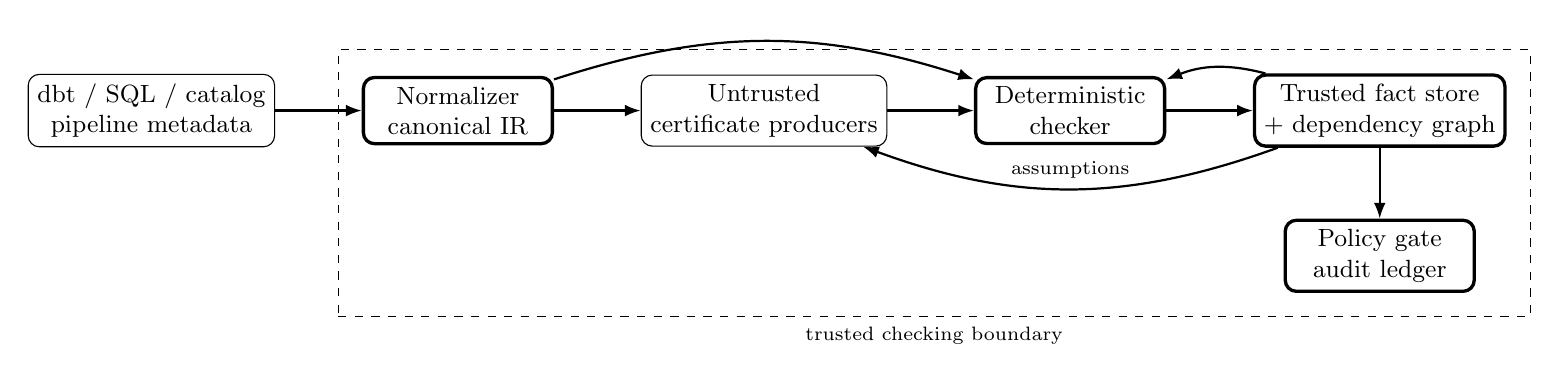
\begin{tikzpicture}[
  node distance=9mm and 11mm,
  box/.style={draw,rounded corners,align=center,minimum height=8mm,minimum width=24mm,font=\small},
  trusted/.style={box,very thick},
  arr/.style={-{Latex[length=2mm]},thick}
]
\node[box] (sources) {dbt / SQL / catalog\\pipeline metadata};
\node[trusted,right=of sources] (norm) {Normalizer\\canonical IR};
\node[box,right=of norm] (prod) {Untrusted\\certificate producers};
\node[trusted,right=of prod] (check) {Deterministic\\checker};
\node[trusted,right=of check] (facts) {Trusted fact store\\+ dependency graph};
\node[trusted,below=of facts] (gate) {Policy gate\\audit ledger};
\draw[arr] (sources) -- (norm);
\draw[arr] (norm) -- (prod);
\draw[arr] (norm) to[bend left=18] (check);
\draw[arr] (prod) -- (check);
\draw[arr] (facts) to[bend left=20] node[above,font=\scriptsize]{assumptions} (prod);
\draw[arr] (facts) to[bend right=18] (check);
\draw[arr] (check) -- (facts);
\draw[arr] (facts) -- (gate);
\node[draw,dashed,fit=(norm)(check)(facts)(gate),inner sep=3mm,label={[font=\scriptsize]below:trusted checking boundary}] {};
\end{tikzpicture}
\caption{CertiFlow architecture. Complex producers remain untrusted; accepted facts can enter the trusted store only through deterministic checker rules.}
\Description{A pipeline metadata source is normalized into canonical IR. An untrusted certificate producer proposes certificates. A deterministic checker validates certificates using the normalized IR and trusted facts. Accepted facts are stored with dependencies and can feed a policy gate and audit ledger.}
\label{fig:architecture}
\end{figure*}

\section{End-to-End Assurance Lifecycle}\label{sec:lifecycle}

Figure~\ref{fig:architecture} separates the pipeline lifecycle into five stages. The separation is not merely organizational: each stage has a different trust obligation.

\paragraph{1. Normalize the pipeline state.}
An adapter converts source artifacts into canonical IR nodes. A node records the operator, normalized arguments, named inputs, engine, and source reference. The canonical hash is therefore a function of the transformation state against which a claim was checked. Engine-specific metadata that cannot be interpreted safely is retained as source context or represented by an opaque node rather than discarded.

\paragraph{2. Seed external evidence.}
Catalog constraints and other administrator-controlled metadata become initial facts. In the live SQLite path, for example, primary-key and unique-index metadata are converted into \texttt{Key} facts. The trust attached to such facts is explicit: CertiFlow's checker can be smaller only if the adapter and the provenance of seed facts are part of the reviewed boundary. A deployment that does not trust a catalog source can instead require a stronger producer or runtime witness.

\paragraph{3. Propose, but do not trust, certificates.}
A producer observes an IR node and the current fact store and emits candidate certificates. The built-in producer is intentionally simple; a future producer could invoke SMT, a proof assistant, a database optimizer, or an LLM. Producer complexity does not enlarge the checker TCB. This distinction is useful for generated data pipelines, where the same probabilistic system that synthesized a transformation should not be allowed to certify its correctness by assertion.

\paragraph{4. Check and compose.}
For each certificate, the checker first validates subject binding and assumption availability, then dispatches a rule-specific obligation. Accepted claims are content-addressed and inserted with explicit dependency identifiers. They can immediately become assumptions for certificates farther downstream. Rejected certificates cannot create facts. Missing evidence yields \textsf{unknown} and therefore cannot satisfy a deployment requirement.

\paragraph{5. Invalidate and gate.}
When pipeline state changes, node hashes identify the changed transformation region and fact dependencies identify the derived evidence that relied upon it. The policy gate evaluates only currently accepted facts. Thus a stale certificate cannot remain effective merely because it was valid for a previous pipeline revision. A hash-chained audit record can retain the sequence of decisions made by the checker.

\subsection{Worked example}

Consider a left join from \texttt{orders} to \texttt{customers} on \texttt{customer\_id}. A live catalog adapter establishes the seed fact
\[
  f_0=\mathsf{Key}(\texttt{customers},\{\texttt{customer\_id}\}).
\]
The producer proposes a \texttt{join\_fanout} certificate whose witness identifies the normalized equality predicate and the right-hand relation. The checker verifies that the predicate in the witness exactly matches the IR and that $f_0$ is present. It can then emit
\[
  f_1=\mathsf{Fanout}(J,\texttt{left\_to\_output},1),\quad D(f_1)=\{f_0\}.
\]
If the join is later edited to use a different right-hand attribute, content binding invalidates the old certificate. Even if a producer re-binds the certificate to the new hash, the semantic rule cannot recover the required right-side key and returns \textsf{unknown} or \textsf{reject}, depending on whether the witness conflicts with the IR or evidence is missing. If the customer key itself is revoked, dependency invalidation removes $f_1$ without requiring an unrelated branch of the DAG to be reconsidered.

\section{Certificate Semantics}

\subsection{Content binding}

Every IR node has a canonical serialization over operator, name, arguments, inputs, engine identifier, and source reference. CertiFlow hashes this serialization with SHA-256. A certificate whose subject hash differs from the current node is rejected before semantic checking. Facts are content-addressed using the same canonicalization contract.

Subject binding solves freshness, not correctness. In the mutation evaluation (Section~\ref{sec:mutation}), every mutant is deliberately re-bound to its new node hash, forcing the semantic rule rather than the freshness check to detect the defect.

\subsection{Rule families}

The current checker registers seven rule families (Table~\ref{tab:rules}). The rules are intentionally small proof obligations over normalized structure and previously accepted facts.

\begin{table}[t]
\caption{Implemented checker rules and their evidence requirements.}
\label{tab:rules}
\small
\begin{tabular}{p{0.28\linewidth}p{0.64\linewidth}}
\toprule
Rule & Checked obligation \\
\midrule
Projection key & Output mapping preserves each column of an accepted input key. \\
Join fanout & Equi-join witness matches normalized predicate and referenced side has an accepted key fact. \\
Group grain & Witness grain equals the normalized grouping key sequence. \\
Restricted flow & Restricted source attributes do not reach prohibited outputs under explicit lineage. \\
Schema compatibility & Actual typed schema satisfies the expected schema relation. \\
Filter key & Selection reissues an accepted input key because filtering cannot duplicate surviving tuples. \\
Union schema & Inputs satisfy the rule's schema-compatibility requirement. \\
\bottomrule
\end{tabular}
\end{table}

For a projection mapping $m$ from output attributes to source attributes, an input key $K=(a_1,\ldots,a_k)$ and proposed output key $K'=(b_1,\ldots,b_k)$ are accepted only when
\[
  m(b_i)=a_i \quad \forall i\in\{1,\ldots,k\}.
\]
For an inner or left equi-join $J=L\bowtie_{L.a=R.b}R$, a trusted key fact $\mathsf{Key}(R,\{b\})$ justifies $\mathsf{Fanout}(J,L\rightarrow J)\leq 1$. If the key fact is absent, the checker returns \textsf{unknown}; it does not assume that observed instance-level uniqueness is an invariant.

Restricted-flow checking uses explicit column lineage. For restricted source set $R_s$ and prohibited outputs $F_o$, the checker rejects if
\[
  \exists o\in F_o:\;\mathsf{lineage}(o)\cap R_s\neq\emptyset.
\]
Lineage for arbitrary expressions is not inferred by this rule; it must come from a trusted normalizer or another checked source.

\begin{proposition}[Relative soundness]
Assume each registered rule is sound for the documented normalized operator semantics and each fact in a certificate's assumption set is valid. If the checker accepts certificate $C$ for node $v$, every emitted claim is valid for the normalized subject represented by the certificate's subject hash.
\end{proposition}

The proposition is relative by design. CertiFlow reduces trust in producers; it does not eliminate the need to validate the checker rules and normalizer semantics.

\subsection{Rule contracts and the trusted computing base}

Each checker rule is a total function over a deliberately narrow input contract. The rule may accept and emit facts, reject malformed or contradictory evidence, or return \textsf{unknown} when required semantics are absent. This contract avoids two common failure modes in assurance tooling: treating missing metadata as a failed property, and treating a successful producer run as evidence that a property holds.

The current TCB consists of canonical serialization and hashing, adapter semantics for trusted metadata, the rule registry and rule implementations, and dependency invalidation. The certificate producer, benchmark generator, LLM assistance, and any future solver are not trusted. This decomposition is useful even before the checker itself is formally verified because it establishes a small auditable target for independent reimplementation. In the current artifact, the semantic checker and model are isolated from the dbt corpus downloader, CLI, and evaluation code.

A further consequence is that claims are \emph{property-specific}. Accepting a join-fanout certificate does not imply arbitrary query equivalence, null-safety, or privacy. The fact store records exactly the property established by the corresponding rule. This prevents a local proof from being interpreted as a global correctness certificate.

\section{Incremental Assurance}

Accepted facts record every fact identifier consulted by their derivation. Let $G_F=(F,E_F)$ be the resulting fact-dependency graph, where $(f_i,f_j)\in E_F$ means that $f_j$ depends on $f_i$. Invalidating root set $R$ removes
\[
  I(R)=\{f\mid \exists r\in R:\;r\leadsto f\}.
\]
The store maintains reverse edges, so invalidation traverses only the dependency closure.

At the transformation level, CertiFlow compares old and new node hashes. Changed nodes and their descendants lose reusable certificates; unrelated branches retain cached evidence.

\begin{proposition}[Selective invalidation]
If each derived fact records every fact consulted by its checker rule, removing $I(R)$ removes all accepted facts whose derivations depend on any invalidated root and preserves every accepted fact outside the dependency closure.
\end{proposition}

This property is operationally important because warehouse DAGs frequently contain independent branches. Revalidating the full graph after a localized change is unnecessary when the evidence dependency graph identifies the affected region.

\subsection{Complexity and reuse}

Let $|V|$ and $|E|$ denote transformation nodes and dependency edges. Canonical hashing is linear in the serialized node size. Topological traversal is $O(|V|+|E|)$. For a changed node set $S$, transformation invalidation traverses the descendant closure $\mathrm{Desc}(S)$ rather than the full graph. Fact invalidation is analogous on the reverse fact-dependency graph. Certificate cache lookup is keyed by the canonical node hash, so an unchanged node can reuse a certificate without reparsing the certificate's source transformation.

This does not imply that every property can be reused solely because the immediate node text is unchanged. Assumption identifiers are part of a certificate, and derived facts depend on those identifiers. A change to an upstream key or schema fact therefore invalidates downstream evidence even when the downstream SQL string itself is byte-for-byte identical. CertiFlow distinguishes \emph{transformation freshness} from \emph{assumption freshness}; both are required for reuse.

\section{Implementation}

The artifact is a dependency-free Python research system. The evaluated revision contains 33 Python source modules and 15 test modules, totaling 2,411 source-and-test lines. The core implementation is divided into canonical hashing, typed models, checker rules, fact storage, DAG and cache logic, adapters, normalization, policy enforcement, and evaluation tooling.

\subsection{Adapters and normalization}

The dbt manifest adapter consumes model dependencies and declared columns. A generic catalog adapter converts engine-neutral catalog rows into scan nodes and trusted seed facts. The live SQLite adapter uses \texttt{sqlite\_master} and \texttt{PRAGMA} metadata to extract schemas, primary keys, and unique indexes without executing user queries.

The SQL normalizer recognizes a documented SELECT fragment covering scans, projections, filters, equi-joins, and grouping. Unsupported relational constructs are rejected rather than guessed. The dbt-aware normalizer preprocesses \texttt{ref()} and \texttt{source()}, decomposes common-table expressions, and preserves unsupported Jinja expressions as opaque computed columns. A macro that generates an entire relation becomes an explicit \texttt{Opaque} IR node. Downstream graph structure is preserved, but no unsupported semantic fact is asserted across the boundary.

\subsection{Verification engine, policy gate, and audit}

The end-to-end engine traverses nodes in topological order. Adapters seed trusted metadata facts. An untrusted inference producer proposes certificates for supported operators. The checker evaluates each proposal and immediately inserts accepted facts, allowing them to serve as assumptions for later nodes.

Deployment requirements can be expressed as predicates over accepted facts. The policy gate therefore consumes the trusted store rather than producer assertions. Verification decisions can also be written to a hash-chained JSONL audit ledger. Each event records the node hash, rule, certificate identifier, verdict, reason, and hash of the previous event. The ledger is not a substitute for external signing, but it makes accidental or post-hoc modification detectable within the recorded chain.

\subsection{Reproducibility surface}

The core has no runtime third-party Python dependencies. The repository exposes unit and integration tests, CLI commands, deterministic mutation workloads, synthetic graph generators, and a pinned real-corpus runner. GitHub Actions executes the test suite on Python 3.9 and 3.12, runs representative benchmarks, verifies the pinned dbt corpus, and compiles the manuscript using the official PVLDB Volume 20 template.

\section{Evaluation}

We evaluate four questions: (RQ1) do the implemented semantic rules reject incorrect witnesses after freshness is neutralized; (RQ2) what is the bookkeeping cost of graph construction and change analysis; (RQ3) how selective is invalidation in a branched DAG; and (RQ4) can the current normalizer represent an unmodified real dbt project while exposing unsupported semantics instead of silently approximating them?

Unless otherwise stated, local timing results were collected with CPython 3.13.5 on Linux 6.18.35 using five virtual Intel Xeon Platinum 8370C cores. Timings are medians of seven runs. The public CI reproduces functional results on Python 3.9 and 3.12; absolute timing values are environment-dependent.

\subsection{Experimental controls and baselines}

The experiments separate three mechanisms that can otherwise be conflated. First, a \emph{freshness baseline} rejects a certificate when its subject hash differs from the current transformation. Second, the semantic mutation experiment neutralizes that baseline by recomputing the subject hash after mutation; any detection is therefore attributable to the rule obligation. Third, the branched-DAG experiment compares dependency-selective invalidation with a conceptual full-revalidation baseline that revisits every node after any change.

We do not report a numerical comparison against dbt tests or contracts because their semantics and configuration are not equivalent to the seven CertiFlow rule families. Such a comparison would require manually aligned invariants and is listed as future evaluation rather than treated as an artificial baseline. The current experiments instead answer whether the implemented checker adds semantic discrimination beyond freshness and whether explicit dependencies reduce revalidation scope.

\subsection{Semantic mutation study}\label{sec:mutation}

We construct valid node/certificate pairs and inject five defect families: wrong join key, wrong aggregation grain, broken key-preserving projection, schema drift, and restricted-field leakage. For each mutant, the certificate is re-bound to the mutant's new subject hash. Consequently, a freshness-only system cannot distinguish the mutant from a newly generated certificate; detection must come from the semantic rule.

\begin{table}[t]
\caption{Semantic mutation results (100 trials per family).}
\label{tab:mutation}
\small
\begin{tabular}{lrr}
\toprule
Fault family & Rejected & Accepted/unknown \\
\midrule
Join key & 100 & 0 \\
Aggregation grain & 100 & 0 \\
Projection key & 100 & 0 \\
Schema drift & 100 & 0 \\
Restricted flow & 100 & 0 \\
\midrule
Total & 500 & 0 \\
\bottomrule
\end{tabular}
\end{table}

CertiFlow rejects all 500 re-bound mutants (Table~\ref{tab:mutation}). This experiment validates the implemented obligations, not real-world recall: the mutants are generated from the same rule families being tested. Its purpose is to show that semantic checking contributes beyond content freshness.

\subsection{Graph scaling}

Table~\ref{tab:scaling} reports deterministic synthetic linear-DAG measurements. The midpoint edit intentionally creates a large descendant set, approaching a worst case for selective invalidation.

\begin{table}[t]
\caption{Median bookkeeping time over seven runs.}
\label{tab:scaling}
\small
\begin{tabular}{rrrrr}
\toprule
Nodes & Build ms & Topo ms & Diff ms & Affected \\
\midrule
100 & 0.27 & 0.09 & 3.15 & 50 \\
1,000 & 2.86 & 1.01 & 32.71 & 498 \\
5,000 & 14.87 & 6.04 & 160.10 & 2,498 \\
\bottomrule
\end{tabular}
\end{table}

The implementation is pure Python and optimized for transparency rather than throughput. Even so, graph construction and ordering remain small relative to typical warehouse execution times. Change analysis scales with the size of the affected region because descendant traversal dominates the midpoint workload.

\subsection{Selective invalidation}

To separate graph size from affected-region size, we construct a root feeding independent branches of fixed depth 100 and modify the midpoint of one branch. With 20 branches (2,001 nodes), 50 nodes are invalidated, or 2.50\% of the graph; median analysis time is 59.3 ms. With 50 branches (5,001 nodes), the same 50-node region represents 1.00\% of the graph; median analysis time is 159.0 ms. A full-revalidation baseline would reconsider all 2,001 or 5,001 nodes respectively.

The main result is not the absolute Python runtime but the reduction in revalidation scope: as independent branches are added, the affected region remains fixed.

\subsection{Pinned dbt corpus}

We evaluate structural normalization on dbt Labs' Jaffle Shop at commit \texttt{7d0d8de2d58edae06f0724a3892da0224bbf0f4a}. The artifact pins the 13 SQL model paths and their Git blob hashes before processing, so an upstream repository change cannot silently alter the workload.

\begin{table}[t]
\caption{Jaffle Shop normalization at the pinned commit.}
\label{tab:jaffle}
\small
\begin{tabular}{lr}
\toprule
Metric & Result \\
\midrule
SQL models & 13 \\
Structurally normalized & 13 \\
Rejected models & 0 \\
IR nodes & 67 \\
Opaque computed expressions & 9 \\
Opaque relation-generating constructs & 1 \\
\bottomrule
\end{tabular}
\end{table}

All 13 models are structurally represented (Table~\ref{tab:jaffle}). Nine dbt/Jinja computations are preserved as opaque computed expressions. One model uses a relation-generating \texttt{date\_spine} macro; CertiFlow retains that CTE as an opaque relation boundary. This behavior is intentional. The system preserves dependency structure while refusing to certify semantics it does not implement.

This experiment measures normalization coverage, not end-to-end proof coverage. A larger study must specify desired invariants for each model and compare CertiFlow against project-specific dbt tests and contracts.

\subsection{Coverage of generated certificates}

On a deterministic 1,000-node synthetic pipeline, the built-in inference producer proposes 502 certificates for operators for which its local rule templates apply. All 502 are accepted and none are rejected or unknown because the workload is generated to satisfy the corresponding rule preconditions. This result is not a recall measurement; it is an end-to-end composition check showing that accepted key and fanout facts become available to later nodes as intended. Mutation testing is reported separately precisely because a positive-path workload alone cannot establish discriminating power.

\subsection{Live SQLite integration}

The integration suite creates a temporary SQLite database with primary and unique-key constraints, extracts the resulting key facts from the live catalog, normalizes a SELECT with a left join and filter, and executes the CertiFlow verification engine. The join-fanout certificate is accepted only because the right-side uniqueness fact is recovered from the catalog. Separate tests exercise composite catalog handling, policy-gate behavior, and the audit-chain invariant. These tests establish an end-to-end path from physical database metadata to accepted downstream facts without hard-coding the key into the certificate producer.

\section{Discussion}

\subsection{Relationship to provenance and formal SQL reasoning}

Provenance semirings and related models characterize derivation at a more general algebraic level~\cite{green2007provenance}; transparent provenance systems capture execution context needed for reproducibility~\cite{rupprecht2020provenance}. CertiFlow uses provenance-like dependency edges operationally to determine which accepted semantic facts become stale. It is not intended to replace provenance systems.

HoTTSQL and axiomatic SQL reasoning provide substantially stronger semantic foundations for supported query fragments~\cite{chu2017hottsql,chu2017axiomatic}. CertiFlow instead defines a small common acceptance interface under which such a prover could act as an evidence producer. Grain-aware verification~\cite{karayannidis2026grain} is particularly close in application domain; CertiFlow generalizes the packaging, trust boundary, and invalidation mechanism across multiple property families.

Data-oriented workflow correctness also requires guarantees spanning individual execution steps~\cite{stonebraker2026workflow}. CertiFlow targets analytical transformation DAGs rather than transactional recovery, but both motivate representing correctness above the level of a single statement.

\subsection{Why three-valued checking matters}

A practical assurance system must distinguish a known violation from missing semantics. Returning \textsf{reject} for every unsupported transformation would make the system unusably conservative; returning \textsf{accept} would be unsound. \textsf{Unknown} allows a pipeline to retain verified facts where evidence exists while exposing precisely where stronger normalizers or producers are required.

The Jaffle corpus illustrates this point. The relation-generating macro is not silently flattened or approximated. Its output remains in the graph behind an opaque boundary, and downstream properties that require its internal semantics cannot be derived without additional evidence.

\subsection{Implications for generated pipelines}

ELT-Bench demonstrates that constructing correct multi-stage pipelines is difficult even for strong code agents~\cite{jin2025eltbench}. CertiFlow does not assume that generated code is trustworthy. An AI system may propose a transformation and separately propose a certificate, but neither receives authority to accept the claim. The checker consumes only normalized structure, trusted assumptions, and a rule-specific witness. This separation is particularly useful when the producer is probabilistic.

\subsection{Deployment semantics}

CertiFlow separates verification from policy. A verifier may accept a narrow fact while a deployment still remains blocked because another required fact is absent. This separation permits different environments to impose different assurance levels without changing rule semantics. For example, a development deployment may permit an opaque model whose outputs are not consumed by a governed dataset, whereas a production gate can require schema and restricted-flow facts for every published relation.

The audit ledger provides tamper-evident chaining within a recorded log, but it is not a secure transparency service by itself. A hostile administrator who can replace both the ledger and its root of trust remains outside the current model. External signing or append-only storage can be layered on the same event hashes when stronger nonrepudiation is required.

\section{Threats to Validity and Limitations}

The current mutation corpus is controlled and aligned with the implemented rules. The 500/500 rejection result should therefore be interpreted as regression evidence for rule semantics, not as an estimate of production defect recall. Naturally occurring faults may be equivalent under SQL semantics, depend on null behavior, or fall outside the current IR.

The Jaffle experiment measures structural normalization of a small but realistic public dbt project. It does not establish complete semantic coverage. A broader evaluation should include multiple independently developed repositories, manually specified target invariants, and comparison with dbt tests/contracts and specialized analyses on their overlapping scopes.

The SQL normalizer is deliberately restricted. Null semantics, collations, casts, window functions, nondeterministic functions, arbitrary UDFs, dialect-specific expressions, and complex set operations require explicit semantics before strong certificates are valid. Opaque boundaries preserve structure but can interrupt proof propagation.

The Python checker is a research reference implementation rather than a hardened security boundary. The correctness propositions are relative to the rule and normalization implementations; they are not machine-checked proofs of the Python code. A smaller independently implemented checker, potentially in Rust or a proof assistant, is a natural next step.

Finally, absolute performance measurements come from a containerized environment and synthetic graphs. The selective-invalidation result is structurally meaningful, but production latency and storage overhead must be measured on larger warehouse DAGs and real CI workflows.

\section{Reproducibility}

The artifact is public at \url{https://github.com/DomTheDeveloper/CertiFlow}. The core experiment commands are:
\begin{itemize}
  \item \texttt{python -m pytest -q} for the 27-test suite;
  \item \texttt{python -m certiflow.bench.evaluate --trials 100} for semantic mutations;
  \item \texttt{python -m certiflow.bench.suite} for repeated scaling measurements;
  \item \texttt{python -m certiflow.bench.branched --branches 50 --depth 100 --repeats 7} for selective invalidation; and
  \item \texttt{python -m certiflow.bench.jaffle} for the pinned Jaffle Shop corpus.
\end{itemize}
The Jaffle runner verifies every upstream Git blob hash before normalization. CI executes the functional suite on two Python versions and compiles this manuscript using the official PVLDB Volume 20 template, which pins \texttt{acmart.cls} v2.19.

\section{Conclusion}

CertiFlow treats data-pipeline guarantees as versioned, machine-checkable artifacts rather than informal assumptions. Certificates are cryptographically bound to normalized transformations, checked independently of their producers, composed through typed facts, and selectively invalidated when their dependencies change. The resulting architecture provides a common acceptance boundary for metadata extractors, static analyses, theorem provers, runtime evidence, and AI-assisted tools without trusting those producers directly.

The current system demonstrates the design across seven semantic rule families, live database metadata, dbt and SQL normalization, incremental graph maintenance, policy enforcement, and a reproducible real-corpus evaluation. The principal open problem is semantic breadth: extending certificate coverage without allowing the checker to grow into another full database engine. The producer/checker boundary is intended to make that extension modular while preserving a small, reviewable source of trust.


\bibliographystyle{ACM-Reference-Format}
\bibliography{certiflow}

\end{document}
